\documentclass{article}
\usepackage{enumerate}
\usepackage{amsmath}
\usepackage{amssymb}
\usepackage{graphicx}
\usepackage{subfigure}
\usepackage{geometry}
\geometry{left=3.0cm,right=3.0cm,top=3.0cm,bottom=4.0cm}
\renewcommand{\thesection}{Problem \arabic{section}.}
\begin{document}

\section{}
\begin{enumerate}[(a)]
	\item
	$$W=-W_G=mg\Delta h=\frac{1}{2}mgl$$
	\item
	$$\int_0^l\mu_0x(l-x)dx=\mu_0(\frac{1}{2}l^3-\frac{1}{3}l^3)=\frac{1}{6}\mu_0l^3=m$$
	$$\mu_0=\frac{6m}{l^3}$$
	$$W=-W_G=\int_0^l\mu_0x(l-x)^2gdx=\mu_0g(\frac{1}{2}l^4-\frac{2}{3}l^4+\frac{1}{4}l^4)=\frac{1}{2}mgl$$
\end{enumerate}

\section{}
	$$G=F_{buo0}=\rho gV=\frac{2}{3}\rho g\pi R^3$$
	$$F=G-F_{buo}=\Delta F_{buo}=\rho g\Delta V=\rho g\int_0^r\pi(R^2-r^2)dr=\rho g\pi(R^2r-\frac{1}{3}r^3)$$
	where r is the distance between the liquid and the medial surface of the ball	
	$$W=\int_0^RFdr=\int_0^R\rho g\pi(R^2r-\frac{1}{3}r^3)dr=\rho g\pi(\frac{1}{2}R^4-\frac{1}{12}R^4)=\frac{5}{12}\rho g\pi R^4$$

\section{}
\begin{enumerate}[(a)]
	\item
	$$W_G=mgx_m$$
	$$W_F=\int_0^{x_m}-kxdx=-\frac{1}{2}kx_m^2$$
	$$W_F=-W_G\Longrightarrow mgx_m=\frac{1}{2}kx_m^2$$
	$$x_m=\frac{2mg}{k}\approx0.0327m$$
	$$|F_m|=kx_m=98N$$
	\item
	$$W_G=mgx_m$$
	$$W_F=\int_0^{x_m}-k(x+160x^3)dx=-\frac{1}{2}kx_m^2-40kx_m^4$$
	$$W_F=-W_G\Longrightarrow mgx_m=\frac{1}{2}kx_m^2+40kx_m^4$$
	$$x_m\approx0.0304m$$
	$$|F_m|=k(x+160x^3)\approx104.7N$$
\end{enumerate}

\section{}
	Suppose a very small distance $dx$ on the x-axis, and the angle between the tangent line of the curve at that position to be $\theta$, then
	\begin{align*}
	f_a&=\mu(mg\cos\theta+F_{ra})\\
	f_b&=\mu(mg\cos\theta)\\
	f_c&=\mu(mg\cos\theta-F_{rc})
	\end{align*}
	where $F_{ri}$ is the centripetal force at that point\\
	And we can find the work done by the friction force in $dx$
	\begin{align*}
	dW_a&=-f_a\frac{dx}{\cos\theta}=-\mu mgdx-\frac{\mu F_{ra}}{\cos\theta}dx\\
	dW_b&=-f_b\frac{dx}{\cos\theta}=-\mu mgdx\\
	dW_c&=-f_c\frac{dx}{\cos\theta}=-\mu mgdx+\frac{\mu F_{rc}}{\cos\theta}dx
	\end{align*}
	Thus the work done by the friction force in the whole procedure is
	\begin{align*}
	W_a&=-\mu mgx-\int_0^x\frac{\mu F_{ra}}{\cos\theta}dx\\
	W_b&=-\mu mgx\\
	W_c&=-\mu mgx+\int_0^x\frac{\mu F_{rc}}{\cos\theta}dx
	\end{align*}
	which means $W_c$ is smallest in magnitude\\
	So path c gives the maximum speed at B.
\section{}
	$$|F|=\frac{x}{L_0}\mu mg$$
	$$W_F=-\int_0^{L_0/2}|F|dx=-\frac{L_0^2}{4}\frac{\mu mg}{2L_0}=-\frac{1}{8}\mu mgL_0$$
	$$\Delta E_k=-W_F\Longrightarrow\frac{1}{2}mv^2=\frac{1}{8}\mu mgL_0$$
	$$v=\frac{1}{2}\sqrt{\mu gL_0}$$
	
\section{}
	$$v'=\frac{vl}{L}$$
	$$m'=\frac{Mdl}{l}$$
	$$dE_k=\frac{1}{2}m'v'^2=\frac{Mv^2l^2}{2L^3}dl$$
	$$E_k=\int_0^L\frac{Mv^2l^2}{2L^3}dl=\frac{1}{3}L^3\frac{Mv^2l^2}{2L^3}=\frac{1}{6}Mv^2$$
	
\section{}
\begin{enumerate}[(a)]
	\item
	$$E_p=\frac{1}{2}kX^2$$
	$$E_k=E_p=\frac{1}{2}mv^2=\frac{1}{2}kX^2$$
	$$v=X\sqrt{\frac{k}{m}}$$
	\item
	$$E_k=E_p=\frac{1}{2}mv^2+\frac{1}{6}Mv^2=\frac{1}{2}kX^2$$
	$$v=X\sqrt{\frac{3k}{3m+M}}$$
	\item
	$$v_a=X\sqrt{\frac{k}{m}}\approx6.143m/s$$
	$$v_b=X\sqrt{\frac{3k}{3m+M}}\approx3.863m/s$$
\end{enumerate}	

\section{}
\begin{enumerate}[(A)]
	\item
	\begin{enumerate}[(a)]
		\item
		$$y=z=0$$
		$$W=\int_{-1}^1F_xdx=\int_{1}^1x^2zdx=0$$
		\item
		$$y=\sqrt{1-x^2}\quad z=0$$
		$$W=\int_a^b(F_xdx+F_ydy)=\int_a^b-xydy=\int_a^b-x\sqrt{1-x^2}d\sqrt{1-x^2}=\int_{-1}^1-x^2dx=\frac{2}{3}$$
		\item
		$$W=\int_a^b(F_xdx+F_zdz)=\int_a^b[t^2(t^2-1)dt+5d(t^2-1)]=\int_{-1}^1t^4-t^2+10tdt=-\frac{4}{15}$$
	\end{enumerate}
	\item
	\begin{enumerate}[(a)]
		\item
		$$y=z=0$$
		$$W=\int_{-1}^1F_xdx=\int_{1}^1-2xdx=0$$
		\item
		$$y=\sqrt{1-x^2}\quad z=0$$
		$$W=\int_{-1}^1F_xdx=\int_{1}^1-2xdx=0$$		
		\item
		$$W=\int_a^b(F_xdx+F_zdz)=\int_{-1}^1-2tdt=0$$
	\end{enumerate}
\end{enumerate}

\section{}
	\indent
	
	(a)
	\begin{figure}[h!]
		\centering
		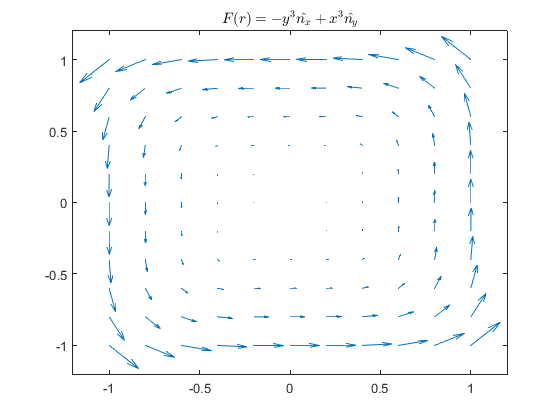
\includegraphics[width=9cm]{p9_1.png}
		\caption{$F(r)=-y^3\hat{n_x}+x^3\hat{n_y}$}
		\label{fig-9-a}
	\end{figure}
	
	(b)
	\begin{figure}[h!]
		\centering
		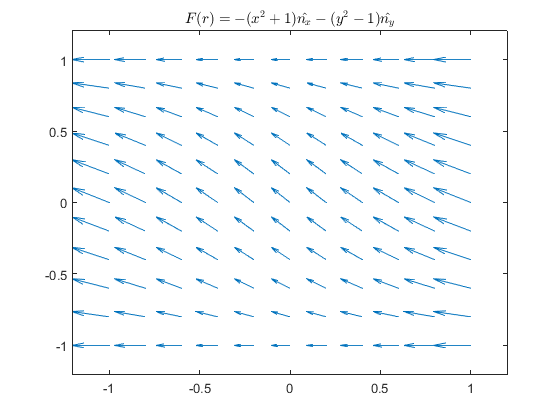
\includegraphics[width=9cm]{p9_2.png}
		\caption{$F(r)=-(x^2+1)\hat{n_x}-(y^2-1)\hat{n_y}$}
		\label{fig-9-b}
	\end{figure}
	
	\newpage	
	
	(c)
	\begin{figure}[h!]
		\centering
		\subfigure[2D]{
		\label{Fig.sub.1}
		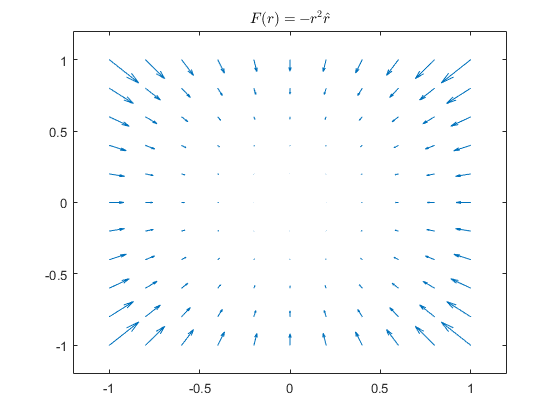
\includegraphics[width=7cm]{p9_3.png}}
		\subfigure[3D]{
		\label{Fig.sub.2}
		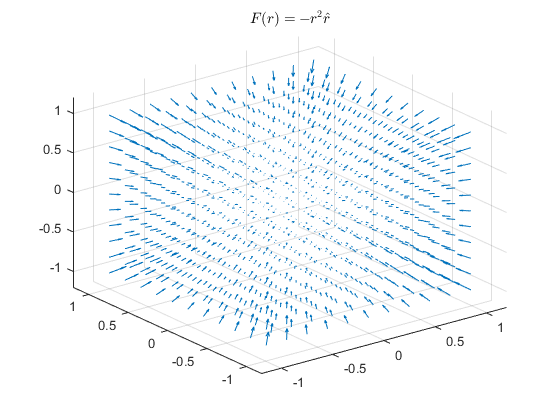
\includegraphics[width=7cm]{p9_4.png}}
		\caption{$F(r)=-r^2\hat{r}$}
		\label{fig-sample}
	\end{figure}

	(d)
	\begin{figure}[h!]
		\centering
		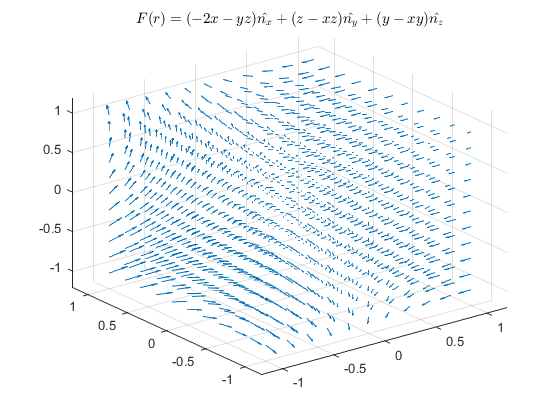
\includegraphics[width=10cm]{p9_5.png}
		\caption{$F(r)=(-2x-yz)\hat{n_x}+(z-xz)\hat{n_y}+(y-xy)\hat{n_z}$}
		\label{fig-9-d}
	\end{figure}

\end{document}
